Pro návrh pásmové propusti 4. řádu s Cauerovou aproximací typu C byly zvoleny parametry tolerančního schématu 
\MapleOutput{f\_s := 80000 Hz}
\MapleOutput{f\_p := 100000 Hz}
\MapleOutput{fp := 877778 Hz}
\MapleOutput{fs := 100000 Hz}
\MapleOutput{ap := 1 dB}
\MapleOutput{as := 80  dB,}
\noindent kde všechny parametry musí být kladná reálná čísla a f\_s <  f\_p < fp < fs a ap < as. Zadána byla spodní a horní hranice nepropustného pásma $f\_s,fs$ [Hz], spodní a horní hranice propustného pásma $f\_p,fp$ [Hz], maximální útlum v propustném pásmu $ap$ [dB] a minimální útlum v nepropustném pásmu $as$ [dB].
\begin{align}
f\_s &= \frac{\sqrt{\Delta{fs}^2+4f\_m ^2}-\Delta{fs}}{2}\\
f\_p &= \frac{\sqrt{\Delta{fp}^2+4f\_m ^2}-\Delta{fp}}{2}\\
fp &= \frac{\sqrt{\Delta{fp}^2+4f\_m ^2}+\Delta{fp}}{2}\\
fs &= \frac{\sqrt{\Delta{fs}^2+4f\_m ^2}+\Delta{fs}}{2}
\end{align}
Funkcí $BP2NLP$ byla provedena transformace tolerančního schematu nesymetrické pásmové propusti (PP) na toleranční schema normované dolní propusti (NDP). Byl spočten geometrický střed propustného pásma $fm$ [Hz], šířka propustného pásma $\Delta{fp}$ [Hz] a šířka nepropustného pásma $\Delta{fs} $[Hz].
\MapleOutput{fm = 141421 Hz}
\MapleOutput{\Delta{fp} = 100000 Hz}
\MapleOutput{\Delta{fp} = 877778 Hz}
\noindent Byl obdržen kmitočet hranice nepropustného pásma normované dolní propusti (NDP) $Os$ [1/s].
\MapleOutput{Os = 8.77778 1/s}.
\begin{figure}[h]
\centering
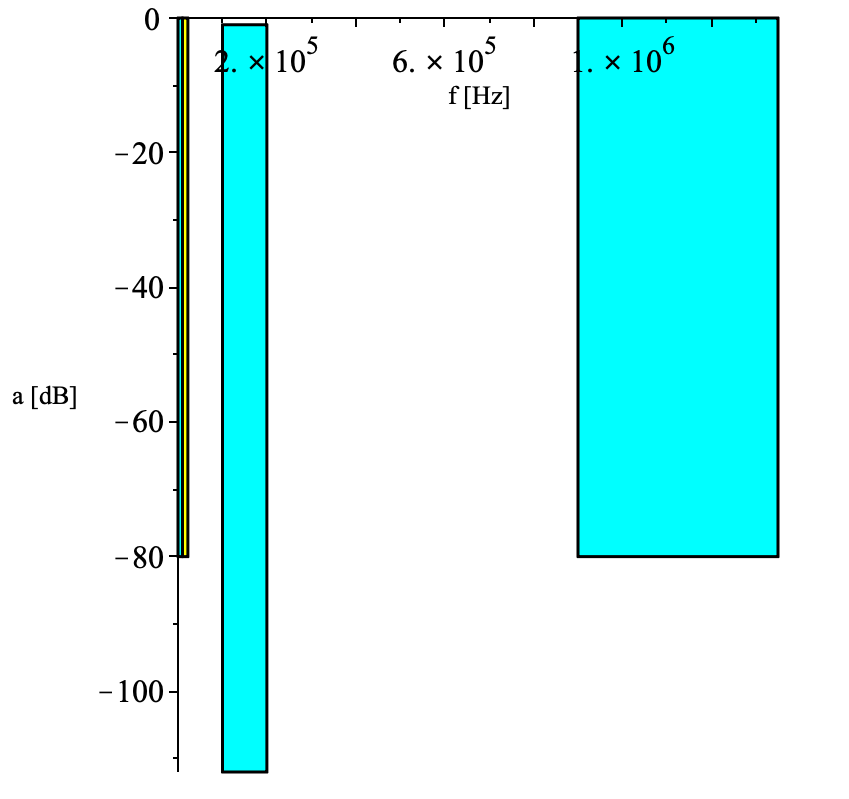
\includegraphics[scale=0.5]{tolsch2.png}
\caption{Toleranční schéma navrhované pásmové propusti}
\end{figure}
\noindent Stupeň Cauerovy aproximace normované dolní propusti byl určen jako $order = 4$.
\noindent Dále byla funkcí $Cauer\_asnew$ určena nová hodnota útlumu v nepropustném pásmu NDP.
\MapleOutput{asnew := 105.613}
\begin{align}
asnew&= 10log10(1 + ( \frac{\epsilon}{kl\_new})^2)\\
\epsilon &= \sqrt{10^{0.1ap} - 1)}\\
k &= \frac{1}{Os}\\
kl\_new &= k^{order}(\prod_{i=1}^{n}JacobiCD(\frac{(2i - 1 + m)EllipticK(k)}{order},k))^4,
\end{align}
\noindent kde $m$ je celočíselný zbytek po dělení řádu 2 a $n$ celočíselný výsledek dělení. Jakobiho eliptických funkcí je 12 a vycházejí ze škálování na jednotkové elipse (cos $\phi$, sin $\phi$ se neváží k jednotkovému kruhu, ale k elipse). $JacobiCD$ funkce je definována jako podíl cosinu Jakobiho funkce s dvěma parametry ($JacobiAM(z,k)$) a derivace této funkce podle prvního parametru z.
\begin{align}
EllipticK(k) = \int _0 ^1(\frac{1}{\sqrt{(-\_ \alpha _1^2+1)}\sqrt{(-k^2 \_ \alpha _1^2+1})})d \_ \alpha _1
\end{align}
Následně byl spočten koeficient nejvyšší mocniny polynomu ve jmenovateli přenosové funkce $Gc$, póly a nuly přenosové funkce $poles, zeros$ pomocí funkce $CauerCPolesZeros$. Počet pólů je dán řádem filtru $order$ a počet nul pro aproximaci typu C je roven $order - 2$. Dále byla spočtena Caurerova aproximace typu C - provozní činitel přenosu $G$ jako racionální lomená funkce $G(j\omega) = 1/H(j\omega)$, charakteristická funkce $chf$ jako $\Phi(j\omega)$ s nulami a póly na imaginární ose a nuly přenosu. Charakteristická funcke má shodný jmenovatel s $G(j\omega)$.
\MapleOutput{Gc, poles, zeros := 376.020,}
\MapleOutput{[-0.475024+0.340009I, -0.475024-0.340009I, -0.162709+0.982758I, -0.162709-0.982758I]),}
\MapleOutput{[11.2840I, -11.2840I],}
\MapleOutput{G,chf,zer := \frac{376.020p^4+479.601p^3+617.689p^2+396.239p+127.328}{p^2+127.329}, \frac{(376.020p^2+311.716)p^2}{p^2+127.329}, [11.2840I, -11.2840I]}
\begin{figure}[h]
\centering
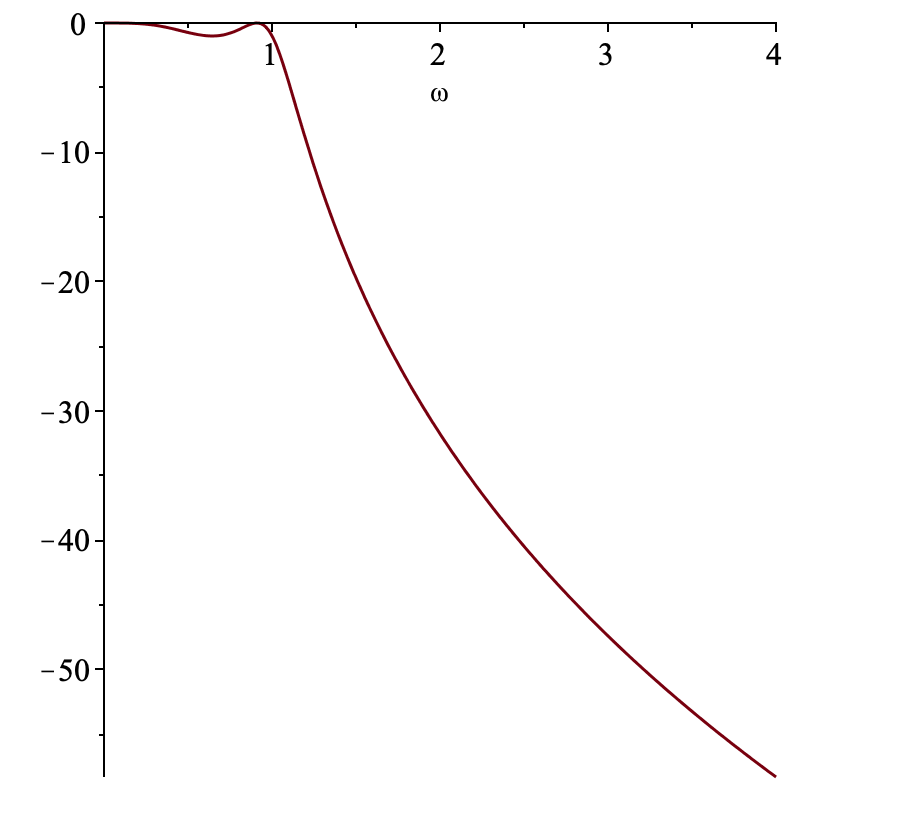
\includegraphics[scale=0.5]{sch02.png}
\caption{Modulová frekvenční charakteristika NDP}
\end{figure}
\noindent Charakteristika byla vykreslena z přenosu funkcí $MagnitudeHdB$, která vypočte modul přenosu podle předpisu |H(j$\omega)$|.
\subsection{Příčkové LC filtry}\label{s:LC}
Pasivní dolní propust je realizována zapojením induktoru ke vstupnímu napětí a k této větvi je následně zapojen paralelně rezistor. Pasivní horní propust má ke vstupu připojený sériově rezistor a poté k této větvi paralelně induktor. \\
K realizaci filtrů vyšších řádů se užívají $\pi$ nebo T články s LC prvky. Při návrhu filtru musí být zohledněn vnitřní odpor zdroje $R_s$ a zatěžovací odpor $R_L$. LC filtry jsou tedy dvojitě zakončeny. Indukčnosti a kapacity prvků se určí z rovnic pro normované kapacity a indukčnosti. Normované hodnoty budou vypočteny pro mezní kmitočet $\omega _c = 1/\sqrt{LC}$ a pro zatěžovací odpor $R_L$. Hodnoty prvků lze pro požadovanou aproximaci odečíst z tabulek. \\
\begin{figure}[h]
\centering
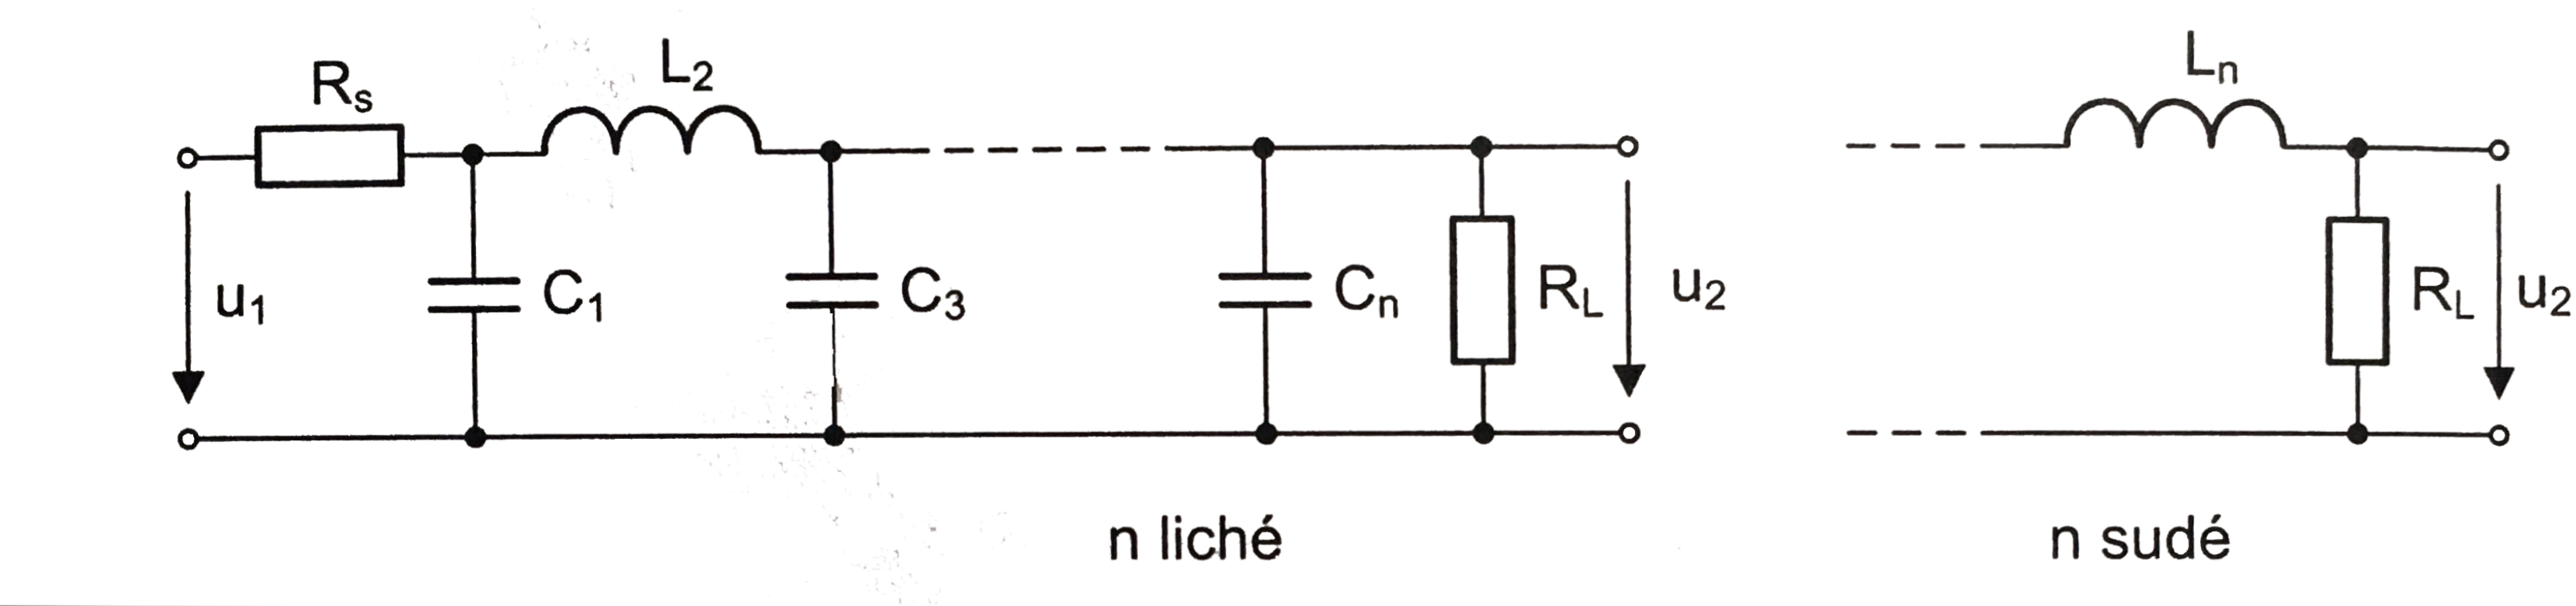
\includegraphics[scale=0.1]{piclanky.png}
\caption[Pasivní dolní propust n-tého řády s $\pi$ články]{Pasivní dolní propust n-tého řády s $\pi$ články \cite{14}}
\end{figure}
\begin{figure}[h]
\centering
\includegraphics[scale=0.08]{tclanky.png}
\caption[Pasivní dolní propust n-tého řády s T články]{Pasivní dolní propust n-tého řády s T články \cite{14}}
\end{figure}
\newpage
\subsection{Gyrátory}\label{s:GYR}
\noindent K převodu induktoru na zapojení s kapacitorem byla použita struktura označovaná jako gyrátor. Jde o náhradu původního obvodu s induktorem vhodným uspořádáním rezistorů a kapacitorů tak, že výsledná impedance vypadá jako induktor. Gyrátor nelze dobře realizovat s obyčejnými operačními zesilovači, běžně se používají /textit{General Impedance Converters (GIC)}. Převod induktoru na jiné zapojení s ekvivalentní impedancí má praktické využití v integrovaných obvodech, kde jsou kapacitory preferovány nad induktory kvůli malým rozměrům. Gyrátor je principielně spojení invertujícího a neinvertujícího napětím řízeného zdroje proudu, a proto ho lze realizovat snadno s transkonduktančními zesilovači. Na Obrázku \ref{s:GO} jsou znázorněny dva gyrátory s kapacitorem. 
\begin{figure}[h]
\centering
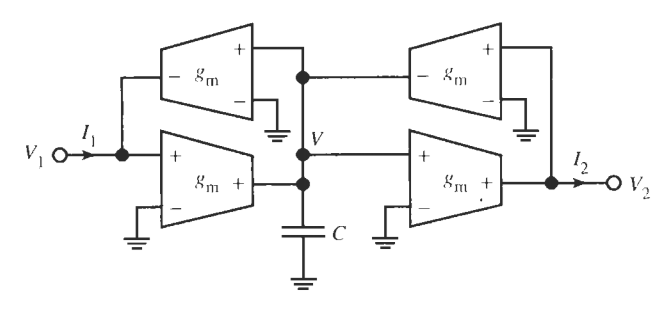
\includegraphics[scale=0.55]{gyrator.png}
\caption[Neuzemněný induktor realizovaný kapacitorem a dvěma gyrátory]{Neuzemněný induktor realizovaný kapacitorem a dvěma gyrátory \cite{12} \label{s:GO}}
\end{figure}
Obvodovou analýzou v uzlu V byla obdržena rovnice
\begin{align}
pCV &= g_mV_1 - g_mV_2
\end{align}
a dva proudy na výstupu
\begin{align}
I_1 = I_2 = g_mV.
\end{align}
Zkombinování rovnic a eliminace V vede k rovnici neuzemněného induktoru mezi napětími $V_1$ a $V_2$.
\begin{align}
I_1 = I_2 = \frac{g_m^2}{pC}(V_1 - V_2) = \frac{1}{pL}(V_1 - V_2)
\end{align}
Z rovnice lze snadno odvodit, že kapacita kondenzátoru použitého při zapojení induktoru s OTA je rovna $C_L = L g_m ^2$. \\
\subsection{Výpočet prvků LC filtru}\label{s:VYP}
\noindent Funkcí $DroppNLP$ byly vypočteny prvky LC příčkového filtru typu normovaná dolní propust (NDP). Zakončení bylo zvoleno standardní (common), odpory o hodnotě 1 $\Omega$, směr zpracování od posledního prvku (rear), s T strukturou (začíná zepředu podélným induktorem). Standardní (common) zakončení je oboustranné ($R_1 \neq 0, R_z \neq \infty$). Výstupem funkce je LC struktura s orientací prvků ve větvi podélně (direct) nebo příčně (shunt).
\MapleOutput{block (1), [orientation = direct, elements = {L1 = -0.40652}, Z = p L1]}
\MapleOutput{block (2), [orientation = shunt, elements = {C1 = 2.4732}, Z = \frac{1}{pC1}]}
\MapleOutput{block (3), [orientation = direct, elements = {C1 = 0.0081309, L1 = 0.96591}, Z = \frac{1}{\frac{1}{pL1} + pC1}]}
\MapleOutput{block (4), [orientation = shunt, elements = {C1 = 1.5489}, Z = \frac{1}{pC1}]}
Vygenerovaná struktura je popsána na Obrázku \ref{s:SCHEM}.
\begin{figure}[h]
\centering
\figppp{Circuit(1)}{5.566}{2.075}{}{}
\caption{Schéma LC příčkové struktury \label{s:SCHEM}}
\end{figure}
\noindent Analýzou LC struktury z Maplu byly obdrženy obvodové rovnice, kde R je volitelný (fiktivní) rezistor:
\begin{align}
I_1 &= \frac{1}{R_1 + pL_1 + \frac{1}{pC_1}}(U_G - U_2)\\
v_1 & = \frac{R}{R_1 + pL_1 + \frac{1}{pC_1}}(U_G - U_2)\\
U_2 &= \frac{1}{\frac{1}{pL_2} + pC_2}(I_1 - I_{3} - I_{L4} - pC_4 v_{L4})\\
U_2 &= \frac{1}{\frac{R}{pL_2} + RpC_2}(v_1 - v_{L3} - v_{L4} - RpC_4 U_{L4})\\
I_{3} &= \frac{1}{pL_3 + \frac{1}{pC_3}}(U_2 - U_3)\\
v_{L3} &= \frac{R}{pL_3 + \frac{1}{pC_3}}(U_2 - U_3)\\
v_{L4} &= \frac{1}{\frac{1}{pL_4}+pC_4}(I_1 - I_{L2} - pC_2U_2 - I_{3} - pC_4 (U_2 - U_3))\\
v_{L4} &= \frac{1}{\frac{R}{pL_4}+RpC_4}(v_1 - v_{L2} - RpC_2U_2 - v_{L3} - RpC_4 (U_2 - U_3))\\
U_3 &= \frac{1}{\frac{1}{R_z}+pC_5 + \frac{1}{pL_5}}(I_1 - I_{L2} - pC_2U_2)\\
U_3 &= \frac{1}{\frac{R}{R_z}+RpC_5 + \frac{R}{pL_5}}(v_1 - U_2 - RpC_2 U_2).
\end{align}
\noindent To odpovídá realizační struktuře s pěti bloky o přenosech $H_1, \ldots,H_5$
\begin{align}
H_1 & = \frac{R}{R_1 + pL_1 + \frac{1}{pC_1}}\\
H_2 &= \frac{1}{\frac{R}{pL_2} + RpC_2}\\
H_3 &= \frac{R}{pL_3 + \frac{1}{pC_3}}\\
H_4 &= \frac{1}{\frac{R}{pL_4}+RpC_4}\\
H_5 &= \frac{1}{\frac{R}{R_z}+RpC_5 + \frac{R}{pL_5}}.
\end{align}
\noindent Uvedené přenosy budou použity v analýze Pracanem.
\noindent Přenosová funkce pasivních a aktivních struktur filtru byla spočtena funkcí $MakeH$. Byl spočten  napěťový i výkonový přenos.
\MapleOutput{H\_NLPV := \frac{p^2  + 127.329}{-193.159 p^4  + 352.072 p^3  + 286.065 p^2  + 582.791 p + 253.653}   }
\MapleOutput{H\_NLP := \frac{p^2  + 127.330}{-96.9631 p^4  + 176.735 p^3  + 143.601 p^2  + 292.553 p + 127.330}}
\begin{figure}[h]
\centering
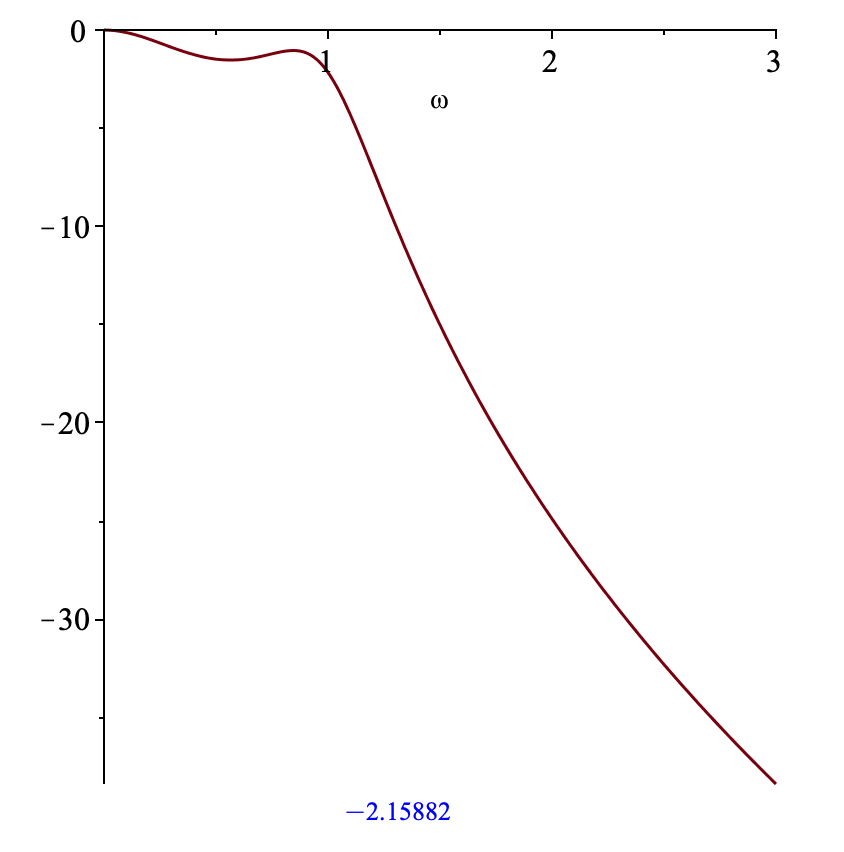
\includegraphics[scale=0.5]{sch022.png}
\caption{Modulová frekvenční charakteristika NDP - LC příčkový filtr}
\end{figure}
\noindent Hodnota přenosové funkce v 1 byla vyhodnocena jako $-2.15882$.\\
Byla provedena transformace hodnot prvků normované dolní propusti (NDP) na pásmovou propust (PP). Zakončovací rezistor byl zvolen 1 $\Omega$, další dva parametry funkce značí spodní a horní hranici propustného pásma.
\MapleOutput{block (1), [Z = p L1 + \frac{1}{pC1}, orientation = direct, elements = { C1 = -7.8301*10^{-6}  , L1 = -3.2350*10^{-7}}]}
\MapleOutput{block (2), [Z = \frac{1}{\frac{1}{pL1}+pC1}, orientation = shunt, elements = {C1 = 1.9681 *10^{-6}, L1 = 1.2871*10^{-6}}]}
\MapleOutput{block (3), [Z = \frac{1}{pC1 + \frac{1}{pL1}+\frac{1}{pL2 + \frac{1}{pC2}}} orientation = direct, elements = { C1 = 6.4704*10^{-9} ,}}
\MapleOutput{C2 = 3.2954*10^{-6}, L1 = 3.9148*10^{-4}, L2 = 7.6864*10^{-7}]}
\MapleOutput{block (4), [Z = \frac{1}{\frac{1}{pL1}+pC1}, orientation = shunt, elements = { C1 = 1.2326 *10^{-6}, L1 = 2.0551*10^{-6}}]}
\noindent Byly nastaveny jakosti cívek v LC příčkové struktuře na konečnou hodnotu. Funkce $MakeRealL$ zařadí do výsledné LC příčkové struktury sériově rezistory k induktorům podle zadaného činitele jakosti $Q$ a zadaného kmitočtu (ten odpovídá u pásmové propusti geometrickému středu propustného pásma - nebo je možno zadat obě hranice propustného pásma). Výpočet sériového odporu je proveden podle předpisu $R_s =L1 \cdot 2 \pi f/Q$.
\MapleOutput{block (1), [Z = p L1 + Rs1 + \frac{1}{pC1}, orientation = direct, elements = { C1 = -7.8301 *10^{-6}, L1 = -3.2350*10^{-7},}}
\MapleOutput{Rs1 = -0.57490*10^{-2}]}
\MapleOutput{block (2), [Z = \frac{1}{\frac{1}{pL1 + Rs1}+pC1}, orientation = shunt, elements = {C1 = 1.9681*10^{-6}, L1 = 1.2871*10^{-6},}}
\MapleOutput{Rs1 = 0.22873*10^{-1}]}
\MapleOutput{block (3), [Z = \frac{1}{pC1 + \frac{1}{pL1 + Rs1}+\frac{1}{pL2 + Rs2 + \frac{1}{pC2}}} orientation = direct, elements = { C1 = 6.4704*10^{-9} ,}}
\MapleOutput{C2 = 3.2954*10^{-6}, L1 = 0.39148*10^{-3}, L2 = 7.6864*10^{-7}, Rs1 = 6.9572, Rs2 = 0.13660*10^{-1}]}
\MapleOutput{block (4), [Z = \frac{1}{\frac{1}{pL1 + Rs1}+pC1}, orientation = shunt, elements = { C1 = 1.2326 *10^{-6}, L1 = 2.0551*10^{-6}, }}
\MapleOutput{Rs1 = 0.36522*10^{-1}]}
\noindent Byl spočten přenos pro LC strukturu bez a s přidanými sériovými rezistory. Pro oba přenosy byla vykreslena modulová frekvenční charakteristika.
\begingroup
    \fontsize{5pt}{12pt}
\MapleOutput{H\_BP := \frac{ p^6  + 2.01858* 10^{14}   p^4  + 1.55854 *10^{23}  p^2}{-6.14026
  10^{-11}  p^8  + 0.000140640 p^7  + 46.6376 p^6  + 5.34196 *10^{8}   p^5 + 2.57033* 10^{14} p^4  + 2.10893 10^{20} p^3  + 7.26886*10^{24} p^2 + 8.65337 *10^{30} p - 1.49149 *10^{36} }}
\MapleOutput{H\_BPQ := \frac{p^7  + 71085.7 p^6 + 2.01860*10^{14}  p^5 + 1.07620*10^{19}p^4+3.47110*10^{23}p^3+6.67244*10^{27}p^2 + 4.92223*10^{31} p}{-6.14027*10^{-11}p^9 +0.000135185 p^8+55.5676 p^7+5.37714*10^8 p^6+2.85360*10^{14} p^5+2.25089*10^{20} p^4+1.49149*10^{25} p^3+8.97641*10^{30} p^2 - 1.38919*10^{36} p - 2.74611*10^{40} }}
\endgroup
\begin{figure}[h]
\centering
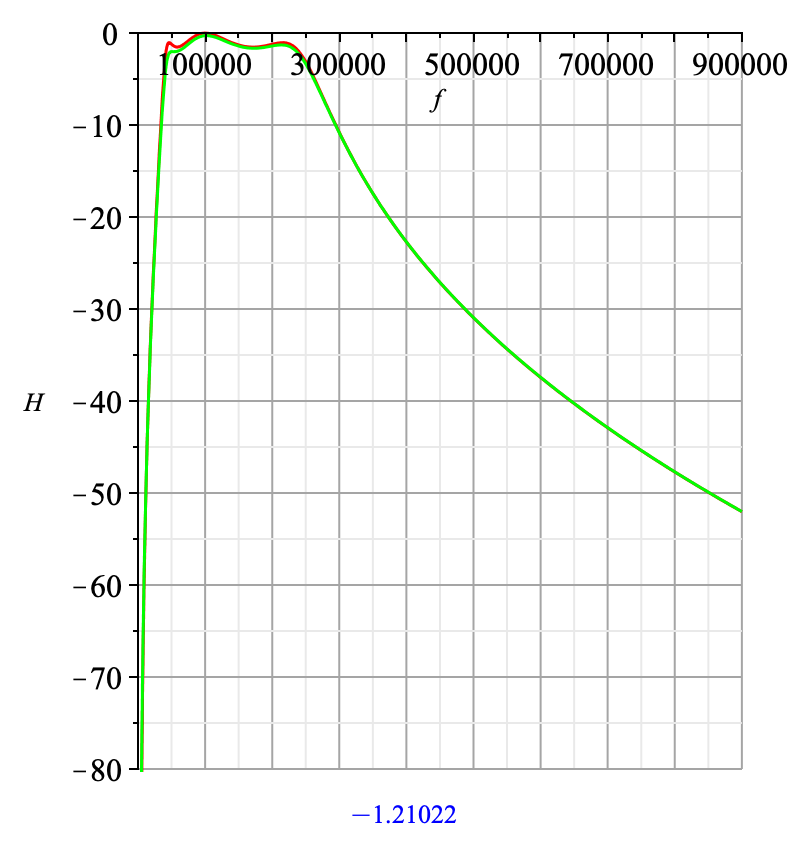
\includegraphics[scale=0.6]{modul12.png}
\caption{Modulová frekvenční charakteristika LC struktury (červená) a LC struktury s konečnou hodntou jakostí cívek (zelená)}
\end{figure}
\noindent Vyčíslením v $200000 \cdot 2 \pi$ Hz byl obdržen útlum 1.21022 dB.\\
\\
\noindent Odnormované prvky byly vyčísleny následovně:
\MapleOutput{ele\_BP := { C1 = -7.83010*10^{-6}  , C2 = 1.96808*10^{-6},  C3 = 3.29545*10^{-6} , C4 = 6.47035*10^{-9},}}
\MapleOutput{ C5 = 1.23258*10^{-6}, L1 = -3.235*10^{-7}, L2 = 1.28706*10^{-6}, L3 = 7.68645*10^{-7}, L4 = 0.391484*10^{-3}, }
\MapleOutput{L5 = 2.05508 *10^{-6}, R1 = 1, Rz = 1.00796}
\noindent Využitím poznatků ze Sekce \ref{s:GYR} byly s uvažováním minimální transkonduktance z datasheetu LM13700 (gm = 9600 $\mu$S) získány kapacity $C_{L1} = 3.08002 $ nF, $C_{L2} = 17.8354$ nF, $C_{L3} = 938.613 $ nF, $C_{L4} = 2.10114$ nF, $C_{L5} = 358.667$ nF.
\noindent Převrácenou hodnotou transkonduktance byly vypočteny frekvenčně a impedančně odnormované odpory
\begin{align}
R_N = R_1 = R_z = \frac{1}{g_m} = 104.16667 \ \Omega.
\end{align}
\noindent Kapacity vyšly již se Syntfilu $C1 = -7.8301 \  \mu$F, $C2 = 1.96808 \  \mu$F, $C3 = 3.29545 \  \mu$F, $C4 = 6.47035$ nF, $C5 = 1.23258 \  \mu$F.
\newpage
\subsection{Návrh funkční simulací}
\noindent  Zapojení s OTA vychází z již uvedených principů v Sekci \ref{s:NAH}. K simulaci byly použity vypočtené hodnoty ze Sekce \ref{s:VYP}. Mezní kmitočet lze přeladit změnou vstupního proudu.
\noindent Bylo použito zapojení se vstupním odporem $R_0$ řazeným paralelně ke zdroji (vhodnější pro funkční simulaci - Schaumann (2001) str. 656/758). Napětí na zdroji poté bude $\frac{V_0}{R_0}$.
\begin{figure}[h]
\centering
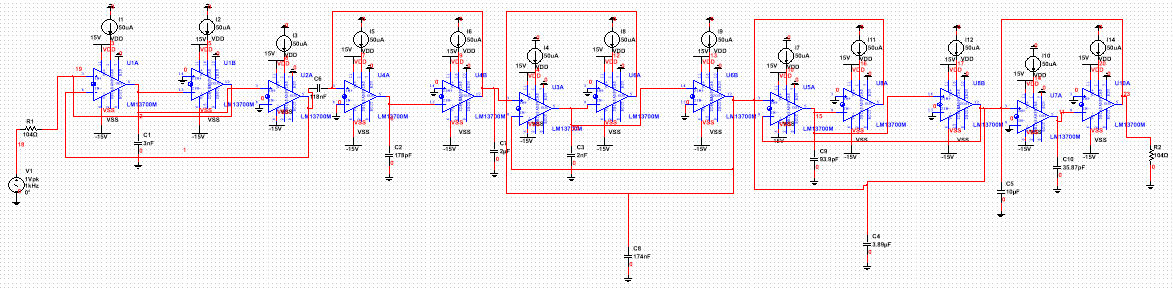
\includegraphics[scale=0.55]{maple.png}
\caption{Výsledné schéma}
\end{figure}
\begin{figure}[h]
\centering
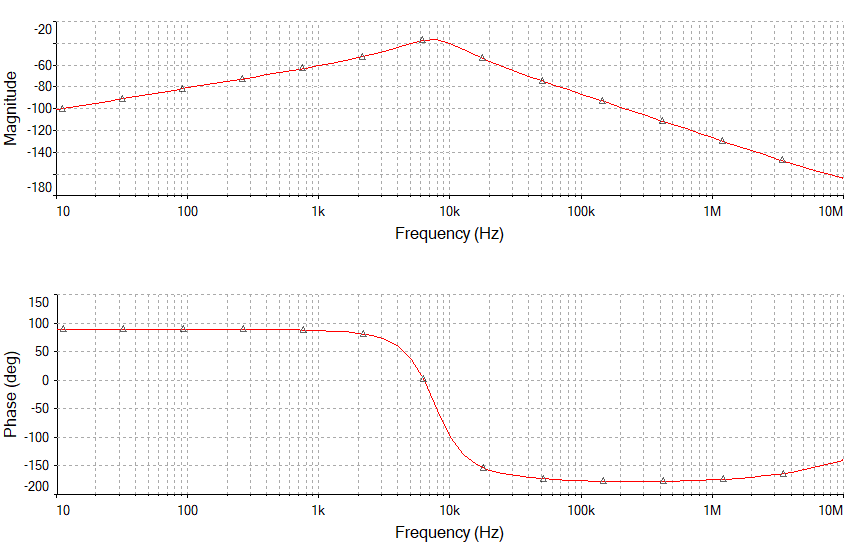
\includegraphics[scale=0.6]{maple2.png}
\caption{Amplitudová a fázová charakteristika PP 4. řádu}
\end{figure}